\documentclass{article}

% http://bayesiandeeplearning.org/
% if you need to pass options to natbib, use, e.g.:
% \PassOptionsToPackage{numbers, compress}{natbib}
% before loading nips_2018

% ready for submission
\usepackage[nonatbib,final]{nips_2018}

% to compile a preprint version, e.g., for submission to arXiv, add
% add the [preprint] option:
% \usepackage[preprint]{nips_2018}

% to compile a camera-ready version, add the [final] option, e.g.:
% \usepackage[final]{nips_2018}

% to avoid loading the natbib package, add option nonatbib:
% \usepackage[nonatbib]{nips_2018}

\usepackage[utf8]{inputenc} % allow utf-8 input
\usepackage[T1]{fontenc}    % use 8-bit T1 fonts
\usepackage{hyperref}       % hyperlinks
\usepackage{url}            % simple URL typesetting
\usepackage{booktabs}       % professional-quality tables
\usepackage{amsmath}
\usepackage{amsfonts}       % blackboard math symbols
\usepackage{nicefrac}       % compact symbols for 1/2, etc.
\usepackage{microtype}      % microtypography
\usepackage{graphicx}
\usepackage{subcaption}
\usepackage{booktabs}
\usepackage{siunitx}

\usepackage[numbers]{natbib}

\title{Metropolitan Generative Adversarial Networks}

% The \author macro works with any number of authors. There are two
% commands used to separate the names and addresses of multiple
% authors: \And and \AND.
%
% Using \And between authors leaves it to LaTeX to determine where to
% break the lines. Using \AND forces a line break at that point. So,
% if LaTeX puts 3 of 4 authors names on the first line, and the last
% on the second line, try using \AND instead of \And before the third
% author name.

\author{
  Ryan Turner \\
  Uber AI Labs
  \And
  Jane Hung \\
  Uber AI Labs
  \And
  Jason Yosinski \\
  Uber AI Labs
}

\renewcommand{\vec}[1]{{\boldsymbol{\mathbf{#1}}}} % vector
\newcommand{\mat}[1]{{\ensuremath{\mathbf{#1}}}} % matrix

\newcommand{\R}{\mathbb{R}}
\newcommand{\D}{\mathcal{D}}
\newcommand{\N}{\mathcal{N}}
\newcommand{\set}[1]{\mathcal{#1}}

\newcommand{\bigO}{\mathcal{O}}
\newcommand{\ceq}{{\stackrel{c}{=}}}
\newcommand{\half}{\frac{1}{2}}
\newcommand{\T}{^\top}
\newcommand{\I}{\mathbb{I}}

\newcommand{\grad}{\nabla}
\newcommand{\sample}{\sim}
\newcommand{\given}{|}

\newcommand{\norm}{\mathcal{N}}
\newcommand{\bern}{\textrm{Bern}}

\DeclareMathOperator*{\argmin}{argmin}
\DeclareMathOperator*{\argmax}{argmax}

\newcommand{\target}{{p^\star}}
\newcommand{\prop}{q}
\newcommand{\pinit}{{p_0}}

\newcommand{\PG}{{p_G}}
\newcommand{\PD}{{p_D}}
\newcommand{\PR}{{p_R}}
\newcommand{\accept}{\alpha}

\newcommand{\setx}{\set{X}}

% Finish clean up checks:
% TODO use smash where needed
% TODO \! arrow where needed
% TODO can search, it is

% TODO add lemma

\begin{document}
% \nipsfinalcopy is no longer used

\maketitle

% Do at end
% Might not be needed for workshop since 3 page limit anyway
% CROP
%\begin{abstract}
%We introduce the Metropolitan Generative Adversarial Network (MGAN), which combines aspect of Markov chain Monte Carlo and GANs.
%The MGAN samples from the distribution implicitly defined by the generator in a GAN\@.
%As such it uses the discriminator from GAN training to build a wrapper around the generator for improved sampling.
%With a perfect discriminator, this wrapped generator samples from the true distribution on the data exactly.
%We demonstrate results on common GAN data sets and wrap the popular DCGAN and WGAN\@.
%\end{abstract}

%\section{Introduction}

% GANs provide implicit way to do density estimation
% traditionally done with explicit likelihood, ancestral sampling in most models to get new synthetic data points from fit model
Generative adversarial networks (GANs) presented a radically new way to do density estimation:
they implicitly represent the density of the data via a classifier that distinguishes real from generated data.
Traditionally, density estimation has been done with a model that can compute the data likelihood.

% GAN uses D and G, but then D usually thrown away
% Use new method to capture knowledge captured in D, to wrap G and create a more intelligent G'
GANs iterate between updating a discriminator $D$ and a generator $G$, where $G$ generates new (synthetic) samples of data, and $D$ attempts to distinguish samples of $G$ from the real data.
Typically, in this setup, $D$ is thrown away at the end of training, and only $G$ is kept for generating new synthetic data points.
In this work we propose the Metropolitan GAN (MGAN) that constructs a new generator $G'$ that ``wraps'' $G$ using the information contained in $D$.
This principle is illustrated in Figure~\ref{fig:block_diag}.

\begin{figure}[bhtp]
    \centering
    \begin{subfigure}[t]{2.25in}
       \centering
       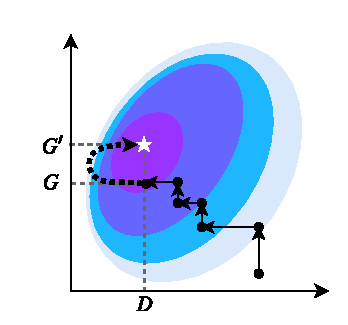
\includegraphics[scale=0.85]{figures/coord_descent.pdf}
       \caption{GAN objective}
    \end{subfigure}
    \hfill
    \begin{subfigure}[t]{3in}
       \centering
       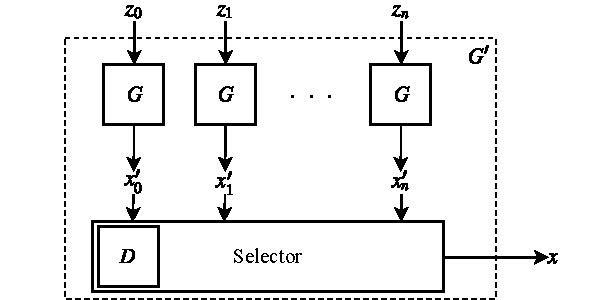
\includegraphics[scale=0.85]{figures/block_diag.pdf}
       \caption{$G'$ wraps $G$}
    \end{subfigure}
    \caption{{\small
    On the left we illustrate how training of $D$ and $G$ in GANs performs coordinate descent on the joint minimax objective, shown in the solid black arrow.
    The final value for the generator and discriminator are denoted $G^\star$ and $D^\star$, respectively.
    If traditional GAN training produces a perfect $D^\star$ for an imperfect $G^\star$, the MGAN wraps $G^\star$ to produce a perfect generator $G'$, as shown in the final dashed arrow.
    On the right we illustrate how the MGAN is essentially a selector among multiple draws from $G^\star$.
    In the MGAN, the selector is built using a Metropolis-Hastings acceptance rule (i.e., MCMC) from the discriminator scores $D^\star$.
    }}
    \label{fig:block_diag}
\end{figure}

% Approach is based on notion that we can sample from real distn \PR implied by D that discriminates between \PR
% Corollary is that if D is perfect, but G is good, we can sample from the data generating distn exactly
The MGAN uses Markov chain Monte Carlo (MCMC) methods to sample from the distribution implicitly defined by the discriminator $D$ learned for the generator $G$.
This is based on the notion that the discriminator classifies between the generator $G$ and a real data distribution:
\begin{align}
  D(\vec x) = \frac{\PD(\vec x)}{\PD(\vec x) + \PG(\vec x)}\,, \label{eq:define PD}
\end{align}
where $\PG$ is the (intractable) density of samples from the generator $G$, and $\PD$ is the real data density \emph{implied} by the discriminator $D$.
If GAN training reaches its global equilibrium then this discriminator distribution $\PD$ is equal to the true distribution on the data ($\PR = \PD$)~\citep{Goodfellow2014}.

% We use MCMC independence sampler to get samples from \PR using multiple samples from G
% MCMC not directly applicable since the likelihood of \PR and G are not available
% However, MCMC only needs the ratio of \PR/G and this can be found from D
We use an MCMC \emph{independence sampler}~\citep{Tierney1994} to get samples from $\PD$ using multiple samples from $G$ (as the proposal)\@.
A corollary is that given a perfect discriminator $D$ and a decent (but imperfect) generator $G$, we can obtain exact samples from the true data distribution $\PR$.
Standard MCMC implementations cannot achieve this because MCMC requires (unnormalized) densities for the target $\PD$ and the proposal $\PG$.
Neither of these quantities are available in GANs.
However, MCMC can be performed using only the ratio $\PD / \PG$, a quantity available directly from the discriminator $D$.

\paragraph{Related Work}
% Need to be clear on diff with NICE-MCMC
A few other works combine GANs and MCMC in some way.
\citet{Song2017} uses a GAN-like procedure to train a RealNVP~\citep{Dinh2016} MCMC proposal for sampling an externally provided target \smash{$\target$}.
The difference is summarized as:~\citet{Song2017} uses GANs to accelerate MCMC whereas we use MCMC to enhance the samples from a GAN\@.
\citet{Kempinska2017} is similar to~\citet{Song2017} but improves proposals in particle filters rather than MCMC\@.

% TODO is this important??
%The GAN approach to density estimation is complementary to the lesser known technique of \emph{density ratio estimation}~\citep{Sugiyama2012}.
%Here, the generator $G$ is typically fixed, or simple, and the density of the data is determined entirely by combining Bayes' rule and the learned classifier $D$.
%In GANs, the key to success is learning $G$ well; while in density ratio estimation the key to success is learning $D$ well.
%The MGAN, in effect, combines elements of both approaches to construct the wrapped GAN $G'$.

\section{Background and Notation}
\label{sec:Background}

\paragraph{MCMC}
MCMC methods attempt to draw a chain of samples $\vec x_{1:K} \in \setx^K$ marginally from a target distribution $\vec x \sample \target$.
We refer to the initial MCMC distribution as $\vec x_0 \sample \pinit$ and the proposal for the independence sampler as $\vec x' \sample \prop(\vec x' \given \vec x_k)=\prop(\vec x')$.
The proposal $\vec x' \in \setx$ is accepted with probability
\begin{align}
  \accept(\vec x', \vec x_k) = \min\left(1, (\target(\vec x')\prop(\vec x_k))/(\target(\vec x_k)\prop(\vec x'))\right) \in [0,1]\,. \label{eq:alpha def}
\end{align}
If $\vec x'$ is accepted then $\vec x_{k+1} = \vec x'$, otherwise $\vec x_{k+1} = \vec x_k$.
We use independent chain for each sample from $G'$.
Each chain samples $\vec x_0 \sample \pinit$ and then does $K$ MH iterations to get $\vec x_K$ as the output of $G'$.

\paragraph{GANs}
GANs implicitly model the data $\vec x \sample \PR$ via a synthetic data generator $G \in \R^L \rightarrow \setx$: $\vec x = G(\vec z)$, $\vec z \in \R^L$.
This implies a (intractable) distribution on the data $\vec x \sample \PG$.
We refer to the unknown true distribution on the data $\vec x$ as $\PR$.
The discriminator $D \in \setx \rightarrow [0,1]$ is a soft classifier predicting if a data point is real.
GAN training forms a game between $D$ and $G$.
If $D$ converges for a fixed $G$ then $D = \PR/(\PR + \PG)$, and if both $D$ and $G$ converge then $\PG = \PR$~\citep{Goodfellow2014}.

In practice, $D$ is often ``ahead'', closer to optimal (\smash{$\PR/(\PR + \PG)$}), than $G$ ($\PR$)~\citep{Shibuya2017}.
This motivates wrapping an imperfect $G$ to obtain an improved $G'$ using a near perfect $D$.

\section{Methods}
\label{sec:Methods}

% Derive basic trick for MCMC using D
In this section we show how to sample from the distribution $\PD$ implied by the discriminator $D$.
If we assume that $D$ is an optimal discriminator between the generator $\PG$ and \emph{some} alternative distribution $\PD$ as per~\eqref{eq:define PD}, we can apply~\eqref{eq:alpha def} for a target of $\target=\PD$ and proposal $\prop=\PG$:
\begin{align}
  \PD/\PG = (D^{-1}-1)^{-1} \implies
  \accept(\vec x', \vec x_k) = \min\left(1, (D(\vec x_k)^{-1} - 1)/(D(\vec x')^{-1} - 1)\right)\,. \label{eq:alpha from D}
\end{align}
If $D$ is perfect then $\PD = \PR$.
This is computable using only the discriminator $D$ and no densities.

\paragraph{Calibration}
A key element is \emph{calibration}: The probabilities for $D$ must not merely provide a good AUC score, but be on the right scale.
%Put in other terms, if one were to warp the probabilities of the perfect discriminator in~\eqref{eq:PD def} it may still suffice for standard GAN training, but it will not work in the MCMC procedure defined in~\eqref{eq:alpha from D}.
We can test the calibration of $D$ using the statistic of~\citet{Dawid1997} on \emph{held out} samples $\vec x_{1:N}$ and real/fake labels $y_{1:N} \in \{0,1\}^N$.
If $D$ is well calibrated: % $y$ is indistinguishable from a $y \sample \bern(D(\vec x))$
\begin{align}
  Z := \frac{\sum_{i=1}^N y_i - D(\vec x_i)}{\sqrt{\sum_{i=1}^N D(\vec x_i) (1 - D(\vec x_i))}} \in \R \implies Z \sample \norm(0,1)\,. \label{eq:calib score}
\end{align}
% This means that large magnitude values for $Z$, i.e., ($|Z| > 2$), reject the hypothesis that $D$ is well-calibrated.
To calibrate $D$, we use a held out calibration set and either logistic, isotonic, or beta~\citep{Kull2017} regression.

\paragraph{Initialization}
We can also avoid the burn-in issues that usually plague MCMC methods.
Recall that via the detailed balance property~\citep[Ch.~1]{Gilks1996}, if the marginal distribution of a Markov chain state $\vec x \in \setx$ at time step $k$ matches the target $\PD$ ($\vec x_k \sample \PD$) then the marginal at time step $k+1$ will also follow $\PD$ ($\vec x_{k+1} \sample \PD$)\@.
In most MCMC applications it is not possible to get an initial sample from the target distribution ($\vec x_0 \sample \PD$), which is usually in \emph{parameter space}.
However, in MGANs, we are sampling from the \emph{data} distribution.
Therefore, by initializing the chain at a sample of real data, we initialize it from the correct distribution and avoid burn-in.

% note how requirement not that strong with calib and manifold
The assumption that $D$ is perfect can be weakened for two reasons:
1)~Because we recalibrate the discriminator, the decision boundaries must be correct, but the probabilities can be suboptimal.
2)~Because the discriminator is only ever evaluated at samples from $G$ or the initial real sample $\vec x_0$, $D$ only needs to be accurate on the manifold of samples from the generator $\PG$ and the real data $\PR$.
This is almost equivalent to saying that the discriminator must rank samples from $G$ (and real samples) the same way that the exact discriminator would.

\section{Results}
\label{sec:Results}

\begin{figure}
    \centering
    \begin{subfigure}[b]{0.32\textwidth}
       \centering
       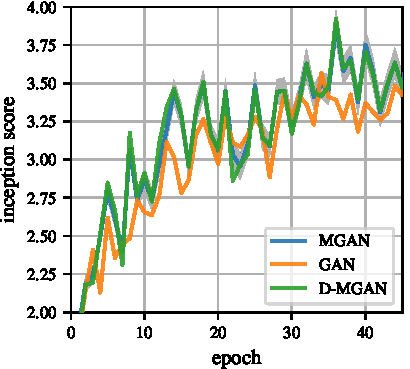
\includegraphics[width=1.8in]{figures/base_iso.pdf}
       \caption{performance by epoch}
       \label{fig:incep_by_epoch}
    \end{subfigure}
    \begin{subfigure}[b]{0.32\textwidth}
       \centering
       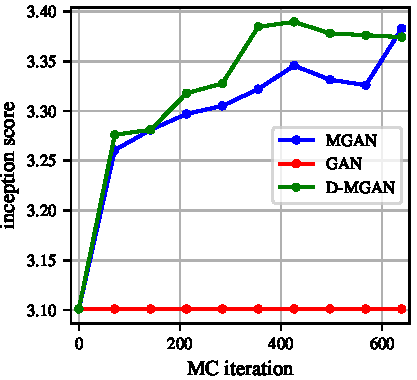
\includegraphics[width=1.8in]{figures/plot_per_mh.pdf}
       \caption{performance by MCMC iteration}
       \label{fig:incep_by_iter}
    \end{subfigure}
    \begin{subfigure}[b]{0.32\textwidth}
       \centering
       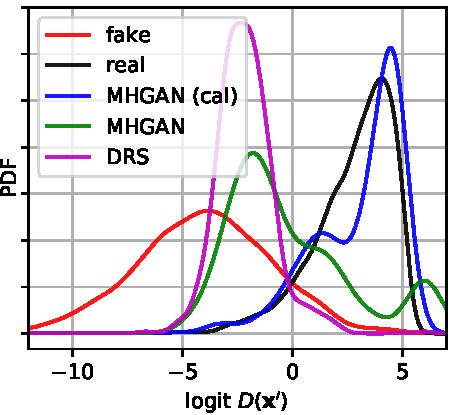
\includegraphics[width=1.8in]{figures/score_dist_overlap.pdf}
       \caption{epoch 13 scores}
       \label{fig:score_dist_overlap}
    \end{subfigure}
    \caption{{\small
    Results of the MGAN experiments on CIFAR-10 using the DCGAN\@.
    On the left, we show the inception score by training epoch of the DCGAN at $K=640$.
    The error bars on MGAN performance (in gray) are computed using a t-test on the variation per batch across 80 splits of the inception score.
    In the center we show the inception score as a function of the number of MCMC iterations $K$ for the GAN at epoch 15.
    On the right we show the scores at epoch 13 where there is some overlap between the scores of fake and real images.
    When there is overlap MGAN can correct the $\PG$ distribution to have scores looking similar to the real data.
    }}
\end{figure}

\begin{table}[htbp]
\centering
    \caption{{\small
    Results showing inception score~\citep{Salimans2016} improvements from MGAN on DCGAN and WGAN at epoch 60.
    Like Figure~\ref{fig:incep_by_epoch}, the error bars and p-values are computed using a paired t-test.
    %All results except for DCGAN on celebA all significant at \smash{$p < 10^{-4}$}.
    We show the MGAN using the raw discriminator scores and the MGAN using the calibrated discriminator scores in ``MGAN (cal.)''.
    }}
    \label{tbl:inception}
{\scriptsize
\begin{tabular}{|l|l|r|l|r||l|r|l|r|}
\toprule
~                 & \multicolumn{4}{c}{DCGAN}                               & \multicolumn{4}{c}{WGAN} \\
\toprule
~                 & CIFAR-10         &      p   & CelebA         &      p   & CIFAR-10        &      p   & CelebA        &       p  \\
\midrule
MGAN              &        3.637(97) &  <0.0001 &      2.374(79) &  0.8584  &              -- &       -- &            -- &      --  \\
MGAN (cal.)       &        3.753(99) &  <0.0001 &      2.58(22)  &  0.0587  &       2.774(64) &  <0.0001 &     2.774(64) &  <0.0001 \\
GAN               &        3.3699(0) &       -- &      2.3676(0) &      --  &       2.5165(0) &       -- &     2.5165(0) &       -- \\
\bottomrule
\end{tabular}
}
% Removed uncalibrated for WGAN since it makes no sense:
% 2.674(61) &  <0.0001 &     2.674(61) &  <0.0001
\end{table}

For real data experiments we considered the CelebA~\citep{Liu2015} and CIFAR-10~\citep{Torralba2008} data sets.
We consider the traditional DCGAN~\citep{Radford2015} and the popular WGAN~\citep{Arjovsky2017}\@.
For WGAN we can only use the calibrated discriminator as it does not output a probability.
%We also show the results of the calibration statistic $Z$ from~\eqref{eq:calib score}.
%These results confirm our expectation that the raw discriminators do not output well calibrated probabilities.

To evaluate the performance of the resulting wrapper generator $G'$, we plot inception scores per epoch in Figure~\ref{fig:incep_by_epoch}.
We see a consistent and statistically significant boost in inception score from $G'$ above $G$.
The actual gap of improvement made by MGAN oscillates from one epoch to the next.
This makes sense as we rely on $D$ being ``ahead'' in some sense.
Because GAN training is a game of sorts, how far ahead $D$ is will vary by epoch.
In Figure~\ref{fig:incep_by_iter} we also plot the inception score per epoch after $K=640$ MCMC iterations.
We see that most of gains are made in the first $k=100$ iterations, but smaller gains continue to $k=400$.

We summarize the performance across all base GANs and data sets in Table~\ref{tbl:inception}.
%The DCGAN and WGAN are shown at epoch 60.
%There was not a substantial difference between different calibration methods, but we found a slight advantage for isotonic regression with the DCGAN and logistic regression for the WGAN\@.
In all cases we ran the MCMC procedure $K=640$ iterations as in Figure~\ref{fig:incep_by_iter}.
We see the same qualitative behavior as in Figure~\ref{fig:incep_by_epoch} with the MGAN correction providing a significant boost in inception score.
Boosts are seen using MGAN from the raw scores, but further improvements are made using the calibrated scores.

% Look at distn on D to make look more like real
%   both on synth and real
In Figure~\ref{fig:score_dist_overlap} we visualize what $G'$ does to the distriubtion on disciminator scores $D$.
We can see that MCMC shifts the distribution of the fakes to match the distribution on true images.
The $Z$ statistic for the raw discriminiator varies from $-77.57$ to $48.98$ over the first 60 epochs; even after Bonferroni correction at $K=60$ we expect $|Z| < 3.35$ with 95\% confidence for a calibrated classifier.
The calibrated discriminator varies from $-2.91$ to $3.60$, which shows it is must closer to calibrated, and therefore unsurprising it boosts performance in the MGAN\@.

\paragraph{Conclusions}
% usual wrap up BS paragraph
We have shown how to incorporate the knowledge in the discriminator $D$ into an improved generator $G'$.
Our method is based on the premise that $D$ is ``ahead'' of $G$.
The principled MCMC setup selects among samples from $G$ to correct biases in $G$.
%We have shown the raw discriminators in GANs are poorly calibrated.
%To our knowledge, this is the first time research has evaluated the discriminator in this way.
This is the first work to rigorously show the poor calibration of the discriminator.
The MGAN has great potential for extension.  % as it performs the final coordinate descent move to optimize $G$ assuming $D$ is near perfect.

\bibliographystyle{abbrvnat}
\bibliography{mgan_refs} % References file

\end{document}

